%%%%%%%%%%%%%%%%%%%%%%%%%%%%%%%%%%%%%%%%%
% Journal Article
% LaTeX Template
% Version 2.0 (February 7, 2023)
%
% This template originates from:
% https://www.LaTeXTemplates.com
%
% Author:
% Vel (vel@latextemplates.com)
%
% License:
% CC BY-NC-SA 4.0 (https://creativecommons.org/licenses/by-nc-sa/4.0/)
%
% NOTE: The bibliography needs to be compiled using the biber engine.
%
%%%%%%%%%%%%%%%%%%%%%%%%%%%%%%%%%%%%%%%%%

%----------------------------------------------------------------------------------------
%	PACKAGES AND OTHER DOCUMENT CONFIGURATIONS
%----------------------------------------------------------------------------------------

\documentclass[
	a4paper, % Paper size, use either a4paper or letterpaper
	10pt, % Default font size, can also use 11pt or 12pt, although this is not recommended
	unnumberedsections, % Comment to enable section numbering
	twoside, % Two side traditional mode where headers and footers change between odd and even pages, comment this option to make them fixed
]{LTJournalArticle}

\addbibresource{sample.bib} % BibLaTeX bibliography file

\runninghead{Shortened Running Article Title} % A shortened article title to appear in the running head, leave this command empty for no running head

\footertext{\textit{Journal of Biological Sampling} (2024) 12:533-684} % Text to appear in the footer, leave this command empty for no footer text

\setcounter{page}{1} % The page number of the first page, set this to a higher number if the article is to be part of an issue or larger work

%----------------------------------------------------------------------------------------
%	TITLE SECTION
%----------------------------------------------------------------------------------------

\title{An Article Title That Spans Multiple\\ Lines to Show Line Wrapping} % Article title, use manual lines breaks (\\) to beautify the layout

% Authors are listed in a comma-separated list with superscript numbers indicating affiliations
% \thanks{} is used for any text that should be placed in a footnote on the first page, such as the corresponding author's email, journal acceptance dates, a copyright/license notice, keywords, etc
\author{%
	John Smith\textsuperscript{1,2}, Robert Smith\textsuperscript{3} and Jane Smith\textsuperscript{1}\thanks{Corresponding author: \href{mailto:jane@smith.com}{jane@smith.com}\\ \textbf{Received:} October 20, 2023, \textbf{Published:} December 14, 2023}
}

% Affiliations are output in the \date{} command
\date{\footnotesize\textsuperscript{\textbf{1}}School of Chemistry, The University of Michigan\\ \textsuperscript{\textbf{2}}Physics Department, The University of Wisconsin\\ \textsuperscript{\textbf{3}}Biological Sciences Department, The University of Minnesota}

% Full-width abstract
\renewcommand{\maketitlehookd}{%
	\begin{abstract}
		\noindent This article presents a mapping of internationalisation and localisation issues in the complex scripts Arabic to give an understanding of the complex script issues in this language. The reason that this article focuses on Arabic localisation is not only that this language is of growing importance as market for many companies.
	\end{abstract}
}

%----------------------------------------------------------------------------------------

\begin{document}

\maketitle % Output the title section

%----------------------------------------------------------------------------------------
%	ARTICLE CONTENTS
%----------------------------------------------------------------------------------------

\section{Introduction}

When software products are developed for distribution in the Arabic speaking regions, technical issues affecting software development and the subsequent localisation process must be considered. Internationalisation and localisation are not just a matter of transferring technology to the business clients in the targeted market. It is also about the cultural conventions that must be handled in computer programs to be able to give all its products the same service, independent of which language the users speak in the 1,500 service workshops all over the world. The goal of this article is to identify some of the issues I come across during whist working on xCP documentum application for Arabic speakers.

\begin{itemize}
	\item The UI should be switched horizontally to the right
	\item The strings have to flow to the right side by applying language direction
	\item CSS should be applied to align the text in the menus
	\item checkbox labels are on the left of the checkbox, and right-aligned
    \item toolbar buttons flow from right to left
\end{itemize}

	Menus
	Messages
	Dialog boxes
	Text direction
	Images
	Toolbars
	Status Bars

\section{Internationalisation}

To be sure that an application can adapted to different countries and cultures, it must be internationalised. We should start by giving a definition of internationalisation what it is made of and what are common issues of applying internationalisation in a software programme. We should also define what is localisation and what the main issue of doing a software localisation in Arabic language. The internationalisation process is handled software engineers and is done at the back up of the application. Engineers add the language identification the HTML scripts 'EN-br' for British English and Fr-fa' for France. For our case study, it is AR-ar which s rather different than the other locales. AR-ar refers to a text that reads from right to left, a text that it is different in script, design, grammar and morphology. AR-ar refers also to a text that must be mirrored to read correctly. When the engineering part of internationalisation is completed, we follow it by adapting the product content to the language and culture of the market.

Did you know that the most widely used writing system in the world after the Latin script is Arabic? The script is used for many languages, often with variations in the way that vowels are represented, or with slightly different repertoires. But what all these languages have in common is that they are read predominantly from right to left. This also has implications for layout: things such as table columns, spreadsheets, graphs, cascading menus, and even web page layout, are normally mirror-images of content produced in English. So instead of using values like 'left' and 'right' in your style sheet, you should use logical values such as 'start' and 'end': that way, when the direction of a page changes, the mirroring happens automatically and without the need for the translator to mess with your code.

Actually, it's even more complicated than that. Arabic mixes right-to-left and left-to-right text on the same line, and it is important to be able to control the direction of the surrounding context for that to work properly. It's also important to handle data strings in a way that preserves information about their base direction, so that when they are used on the user interface they don't look mangled.

You will usually want to store data internally in one standard form, but display it in ways that look natural to local users. As well as the names and addresses already mentioned, does the person working with your app or content expect to see periods or commas for decimal points? How about the order of day, month, and year, or even which day begins the week in a calendar?

\subsection {Time zones, currencies, dates}

You may also need to support alternative calendars, time zones and daylight savings, in both native plus transliterated forms, etc. Did you know that there are numerous countries around the world that have local calendars, and use them on a regular basis? Birth dates are typically recorded in the Imperial calendar in Japan, and newspapers in Thailand usually carry the date in the Buddhist calendar (the Western year 2022 is 2565 in Thailand). Any app you create needs to be able to adjust information for the appropriate time zone.

If working with monetization, you'll need to consider how to handle users who work with a range of currencies. In addition to deciding how to format and represent monetary data when displayed to the user, you also should consider how to put in place mechanisms to manage diverse currency systems. How will you develop pricing models for different countries, which may have large variations in standard of living? How will you convert subscriptions and payments from one currency to another?

\subsection{Text Direction}

One of the biggest concerns with Arabic localization is text direction. Arabic is considered a “bi-directional” language using right-to-left (RTL) script likewise “Hebrew” and “Urdu”. Moreover, For Right-To-Left (RTL) languages, not only does the text alignment and text reading order go from right to left, but also the “UI” elements layout should follow this natural direction of going from right to left. Linear layout from left-to-right cannot be assumed in complex scripts. Chinese can be written horizontally or vertically, but it is considered to be unidirectional because it does not mix directions in the same text. Arabic is bidirectional, since text in the Arabic script is written from right-to-left but numbers and characters in the Latin script in the same text are written from left-to-right. Because the direction of text may change from one character to the next in Arabic, text handling procedures must be available in both right-to-left and left-to-right text. Text is usually stored in a single, logical progression in a computer, and special rendering algorithms make the direction of display and printing of the text bidirectional. Character reordering is when characters in sequence are rearranged from the logical keystroke order18 to their visual order19. Graphics and icons are also affected by text direction. In an Arabic graphical user interface even the layout of items such as tables and charts are typically mirror imaged on the horizontal plane.

%------------------------------------------------

\subsection{Content Customisation}
\section{Translation}

Translation also was not looking consistent and I had to go through the application to check it and come up with a better translation according to the context.
Finally and Based on the elements mentioned above, I have suggested the followings the followings solutions:

There are two ways to work out this process. If the application content is not massive, the company can hire a team of linguists to help with the content translation, the linguist can translate the content directly inside the 'html' or 'xml' scripts without moving the text outside the application. There are many tools offering that. e.g OxygenXML is offering the facility of editing the text inside the editor. This process is not easy in itself because it requires the linguists to have a good knowledge of the  software industry. They should know how to move between the code editor and the visual editor, how to run regressive test scenarios and who to write an SQL script. They should also know where the application segments sit on the system.

The second option is to extract the content from the scripts, add it to an excel spreadsheet while creating different text columns, one for the source text and another one for the targeted text, then request the language vendor to take in charge the content translation. There are some drawback with this second option. The language vendor is usually a consultancy, a business. They are using the service of independent linguists who when they work with a segment of a text neglect the context of the text they are translating. Translation errors and a loss of consistency is an error some language vendors fall in.

The localisation of a software application is a mandatory task for any business seeking an expansion to other markets. It is also an obligation in some countries. In Europe and in order to respect the legal convention, it is an obligation for any company seeking to commercialise its product outside its national borders to translate and localise the content of its products, including but not limited the product description, the product labels, the packaging and the website displaying the product. This is usually done for the product reference. All those tasks must be completed before the commercialisation and advertisement the product. In Europe for example, consumers cannot purchase a product that does not speak the local language. This is usually done for the safety of the consumer and for the legal protection of the business. If a consumer buys a product of which the content is written in another language, they can fall in the error of buying a product that is not suitable for them and any consequences resulting from the wrong usage of the product will be handled by the business that manufactures, sells and advertise the product. Businesses prefer not to engage in legal issues because it is against the market reputation.

\subsection {Language scope}

Cultural The third task included in the localisation of a product, is the cultural adaptation. Countries have different cultural ties. This is why the product advertised must respect those conventions. A concrete example of this can be found in the Arab world where Arabic countries use the Modern standard form of Arabic MSA as a language of the media and spoken forms of Arabic for daily conversations. There are many variations of Arabic  \href{https://en.wikipedia.org/wiki/Varieties_of_Arabic}{variations} and a term can mean different things according to user's location. In Egypt for example, speakers say /kazouza/ to name a fresh drink. In Morocco, the term used is /lmonada/ a term that has been borrowed from the French dictionary /Limonade/ and was customised to the Moroccan tongue.

\subsection {Multi-level baselines}

Letters may join through a finely inclined line.

Multi-context joining

Vertical joining


 Bidirectional text

You'll also want to do some homework in advance about the cultural preferences and habits of the marketplaces where you want your application to be used, and choose flexible content design technologies and processes so that you can later support others.

For example, symbolism can be culture-specific. The check mark means correct or OK in many countries, but in some countries, such as Japan, it can be used to mean that something is incorrect. Japanese localizers may need to convert check marks to circles (their symbol for 'correct') as part of the localization process.

use  are usually used inside the national borders. of a unless they are sure such as In this process, we should extract all And then it has to be adapted, localised, to each specific customer’s local cultural requirements. From my long experience working in the field of language industry, I have come across three type of software localisation product. I would like to show some examples in the graphs below

\begin{figure}
    \centering
    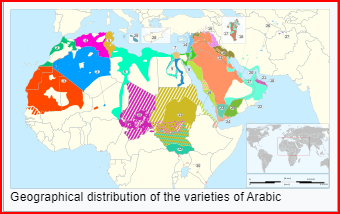
\includegraphics[width=0.5\linewidth]{Arabic variations.png}
    \caption{Enter Caption}
    \label{fig:enter-label}
\end{figure}

\section {Arabic Layout Requirements}

\subsection{Limitations}

This thesis focuses on the language handling that can be seen in the graphical user interface and primarily of the Chinese and Arabic scripts. It does not include any technique for translation or how this should be treated. Neither does this thesis include anything about fonts, even though the availability of fonts is one of the most critical aspects of displaying or printing text in a complex script. (Without adequate font support a fully functional complex script-capable application is completely worthless). But font issues are such a large and time consuming topic, not possible to be handled within the time frame of this thesis, and are therefore considered to be out of scope. Because of the same reasons this thesis is limited to a “script-technical focus”, not a “cultural focus” (even though “culture” is mentioned in the 
thesis). It does not either discuss the distinction between a script versus typography, since typography is very culture-dependent.

\subsection{Handling Direction-Sensitive Graphics}

Direction-sensitive graphics (such as bitmaps and icons) present another challenge with regard to mirroring. Some direction-sensitive graphics can have a different meaning when mirrored. For example, within an LTR layout in a browser, an arrow that points to the left represents the concept of going back to the previous page; an arrow that points to the right would signify going forward to the next page. When these arrows are mirrored for an RTL layout, the meaning will be just the opposite. The direction of writing affects the way information should be presented and placed. For example, some applications use icons to tell users to go to the "Next" or "Previous" page. Because these icons do not have the same meaning when used with a bidirectional language, however, users often become confused (Figure 1). 

%------------------------------------------------

\subsection{Alignment and Formatting}

Written content should be aligned to properly display and wrap text at the end of each sentence. If not, the order of the words and the meaning of the sentence will be incorrect. Fortunately, most applications have tools that can change the writing direction of the text. For example, markup languages like HTML have tags you can add to your code to adjust the "DIR attribute" and specify the base direction of text (LTR, RTL). Based on the elements mentioned above and the design of EMC Europe (see example below) I have come with the following conclusions. The application should be redesigned completely because it is, from a user perspective, look faulty. Moreover, in EMC application we cannot distinguish between attributes, which attribute is a parent attribute and which attribute is a child. Seeing the fact that the design Seeing the fact that the layout is not looking correct, a user cannot distinguish between attributes, which attributes is a “Parent” attribute and which attribute is a “Child” attribute. I am attaching an example for more clarification of the case.

This line shows how to use a footnote to further explain or cite text\footnote{Example footnote text.}.

\subsection{Confirmation Messages /Error Messages}

During my work on both application xCP and Record Manager, I have realized that Error/Confirmation messages were returning corrupted and thus incorrect. I have suggested on them a solution that has worked efficiently. 

\subsection{International Support}

\noindent m

\noindent À

\noindent ßÇŒÆČŠŽ

\subsection{Links}

This is a clickable URL link: \href{https://www.latextemplates.com}{LaTeX Templates}. This is a clickable email link: \href{mailto:vel@latextemplates.com}{vel@latextemplates.com}. This is a clickable monospaced URL link: \url{https://www.LaTeXTemplates.com}.

%------------------------------------------------


\subsection{Subsection One}

Suspendisse

\subsection{Subsection Two}

Nullam

\subsubsection{Subsubsection Example}
 

%----------------------------------------------------------------------------------------
%	 REFERENCES
%----------------------------------------------------------------------------------------

\printbibliography % Output the bibliography

%----------------------------------------------------------------------------------------

\end{document}
